\documentclass[runningheads]{llncs}

\usepackage[T1]{fontenc}
\usepackage[utf8]{inputenc}
\usepackage{graphicx}
\usepackage{amsmath}
\usepackage{amssymb}
\usepackage{booktabs}
\usepackage{multirow}
\usepackage{xcolor}
\usepackage{threeparttable}
\usepackage{subcaption}
\usepackage{float}
\usepackage[section]{placeins}

\begin{document}

\title{MESC-DAST: A Unified Framework for Medical Image Classification and Grading}
\titlerunning{MESC-DAST}

\author{Anonymous ICIG Submission}
\authorrunning{Anonymous}
\institute{Anonymous Affiliation}

\maketitle

\begin{abstract}
Medical image classification and grading remain challenging due to low contrast, complex lesion morphology, class imbalance, and pronounced multi-scale structural variations. Ordinal medical grading tasks further contain structured inter-class relationships that are not directly captured by conventional one-hot supervision. To address these issues, we propose a unified ResNet50-based framework that combines a Median-enhanced Spatial and Channel Attention (MESC) module with a Distance-Aware Soft Target (DAST) loss. MESC is a plug-in feature enhancement module that fuses average, maximum, and median channel statistics and then applies multi-scale depthwise spatial modeling. DAST is a training-time supervision objective that constructs class-distance-decayed soft targets over the original softmax output. Experiments on HAM10000, Chest X-ray Image, ADNI-derived Alzheimer MRI, Brain Tumor MRI, and Knee Osteoarthritis datasets show favorable performance among the evaluated baselines. The ablation study indicates that MESC provides stable gains across several datasets, while DAST is most beneficial when the label space has a clear ordinal structure, such as Knee Osteoarthritis grading. These results suggest that combining robust feature recalibration with distance-aware supervision is a practical strategy for medical image classification and grading, while broader multi-seed validation remains an important direction for future work.

\keywords{Medical image classification \and Medical image grading \and Attention mechanism \and Soft target loss}
\end{abstract}

\section{Introduction}

Medical image analysis is an important application of computer vision and plays a crucial role in disease screening and graded diagnosis. In recent years, deep learning methods, especially Convolutional Neural Networks (CNNs), have made significant progress in this field \cite{1}. However, different from natural image classification tasks, medical grading problems usually have more complex structural characteristics: on the one hand, lesion regions often exhibit features such as low contrast, irregular morphology, and significant noise interference, which pose higher requirements for the model's feature extraction ability \cite{1,23,27}; on the other hand, different classes usually have a clear ordinal structure, for example, in Kellgren--Lawrence (KL) grading, the differences between adjacent grades are often subtle, while those between distant grades are clearly distinguishable \cite{2,3,10}.

Most existing methods are modeled based on standard CNN backbones (such as ResNet) \cite{4}, and enhance feature representation ability by introducing attention mechanisms or multi-scale structures \cite{5,6,7,8,13,14,15,16}. However, such methods typically rely on simple statistics such as average pooling or max pooling to construct attention weights \cite{5,6}, which can easily lead to unstable feature estimation in the presence of noise or abnormal responses. Meanwhile, although multi-scale modeling can enhance the model's perception of different structures to some extent \cite{7,8,13,14}, it often lacks effective constraints on the relationships between scales during the feature fusion process, resulting in the model's generalization ability still being limited in complex medical scenarios \cite{8,23}.

On the other hand, in the design of loss functions, most methods still use one-hot labels combined with cross-entropy loss for training, treating each category as an independent discrete label \cite{9,10}. This modeling approach ignores the ordinal relationship between categories, preventing the model from distinguishing between "adjacent category errors" and "long-distance errors" during the optimization process, thus limiting its performance in medical grading tasks \cite{3,9,10}. Although existing studies have attempted to introduce certain structural information through methods such as label smoothing or ordinal regression \cite{9,10,11}, and further combined uncertainty modeling or soft label supervision in medical tasks to alleviate the limitations imposed by hard labels \cite{22,25,26,27}, it remains difficult to strike a good balance among expressiveness, structural modeling ability, and implementation complexity \cite{10,23,25}.

To address the above issues, this paper proposes a unified optimization framework from two aspects: feature modeling and loss function design. Specifically, we introduce a Median-enhanced Spatial and Channel Attention (MESC) module into the middle and high layers of the residual network. By combining multiple statistical information and multi-scale spatial modeling, we enhance the robustness and discriminative ability of feature representation. Meanwhile, we design a Distance-Aware Soft Target Loss function, which explicitly encodes the distance relationships between classes, enabling the model to better reflect the structural characteristics of medical grading tasks during the training process.

The main contributions of this paper are as follows:
\begin{enumerate}
    \item A Median Enhanced Spatial Channel Attention Module (MESC) is proposed. This module introduces median pooling in channel attention to enhance robustness against noise, and combines multi-scale depth convolution to effectively model spatial features, thereby obtaining more stable and discriminative feature representations in complex medical images.

    \item A Distance-Aware Soft Target Loss function is proposed. This method constructs a soft target distribution based on category distance decay, enabling the model to distinguish different degrees of classification errors, thus better meeting the actual requirements of medical grading tasks.

    \item The effectiveness of the proposed method is evaluated on multiple medical image datasets. The results show that the method improves over the ResNet50 baseline under the same experimental setting and achieves competitive performance among the evaluated baselines.
\end{enumerate}

\section{Related Work}

The proposed framework is related to two lines of work: attention-based feature enhancement and structured supervision for ordered labels. Unlike works that only replace the backbone or add a generic attention block, our focus is on a controlled ResNet50 setting in which the feature module and the loss function can be independently ablated.

Convolutional Neural Networks (CNNs) have long dominated Computer Vision tasks, particularly in medical image analysis, where they demonstrate strong feature extraction capabilities\cite{1}. Represented by ResNet proposed in Deep Residual Learning for Image Recognition, the introduction of residual connections effectively alleviates the vanishing gradient problem in deep networks, enabling a significant expansion of network depth and thus bringing continuous performance improvements \cite{4}. On this basis, subsequent research generally adopts the approach of introducing lightweight modules into the ResNet backbone structure to enhance representational ability, such as embedding feature enhancement units in the middle and high-level feature stages (e.g., layer3, layer4), to improve the modeling ability of complex patterns while controlling computational overhead \cite{5,6,7,8,15}. However, traditional residual structures still essentially rely on local convolution operations, with limited ability to model long-range dependencies and global context; to alleviate this issue, subsequent research has introduced mechanisms such as non-local operations to explicitly capture long-range dependencies \cite{16}. This limitation is particularly prominent in medical image scenarios, as lesion regions typically exhibit characteristics such as cross-scale distribution, low contrast, and strong noise interference \cite{1,23,27}.

To address the limitations of CNNs in global modeling, attention mechanisms have been widely introduced into visual models. Channel attention methods, such as Squeeze-and-Excitation Networks, recalibrate features by modeling inter-channel dependencies \cite{5}; spatial attention methods, such as CBAM, further incorporate spatial dimension information to enhance the response of key regions \cite{6}. These methods have achieved significant performance improvements in natural image tasks and have gradually been transferred to medical grading tasks, such as attention-based KL grading models and multi-scale knee osteoarthritis grading networks that incorporate attention mechanisms \cite{7,8}. In addition, for the automatic grading of knee osteoarthritis, researchers have also proposed frameworks based on Siamese CNN, ensemble learning, and multi-stage processing workflows to improve the recognition accuracy and stability of KL grading \cite{18,19,20,21}. However, existing attention mechanisms typically rely on limited statistical descriptions, such as average pooling or max pooling, to generate attention weights \cite{5,6}; in the presence of noise or abnormal responses, this design is prone to unstable attention estimation. Moreover, their spatial modeling capabilities are often limited to a single scale or shallow convolution structures, making it difficult to fully characterize the multi-scale structural features in complex medical images \cite{6,7,8,13,14}.


Multi-scale modeling, as an important direction for enhancing the expressive power of visual models, is particularly crucial in medical image analysis because lesion regions often exhibit significant scale variations \cite{1}. Early methods such as the Inception series achieved feature fusion through parallel multi-scale convolution branches \cite{13}, while subsequent work more often adopted depthwise separable convolution to reduce computational complexity while maintaining expressive power, with typical representatives including Xception and MobileNetV2 \cite{14,15}. In recent years, some studies have attempted to combine multi-scale convolution with attention mechanisms to achieve better performance in complex scenarios \cite{7,8,20,22}. For example, in the knee osteoarthritis grading task, the method based on attentive multi-scale CNN has demonstrated that the fusion of multi-scale and attention helps improve the representation ability for different structural scales \cite{8}. However, existing methods often lack effective structural constraints during the multi-scale feature fusion process, making it difficult to adaptively adjust the contributions between features of different scales, and they are still relatively sensitive to noise in high-resolution medical images, which limits their stability and generalization ability in actual clinical scenarios \cite{8,20,23}.


In medical grading tasks, especially Kellgren–Lawrence grading, there is usually a natural ordinal structure among classes \cite{2,3,10,18,19,20,21,22}, yet this structure is often overlooked in traditional classification frameworks. Mainstream methods typically use one-hot labels combined with cross-entropy loss for training, causing the model to treat each class as an independent discrete label \cite{9,10}. To alleviate this issue, some studies introduce label smoothing to soften the label distribution, thereby reducing the risk of overfitting \cite{11}, but it still fails to capture the structural relationships among classes; Focal Loss improves model performance by reweighting hard samples \cite{17}, but also does not explicitly model the distances between classes; while methods based on ordinal regression or ordinal regularization improve medical grading performance by explicitly utilizing class order information \cite{3,9,10}, but usually introduce additional modeling complexity. Overall, although these methods improve classification performance to some extent, they still fail to effectively model the "distance semantics" between classes and struggle to distinguish between adjacent class errors and long-distance errors.

DAST differs from these supervision strategies in its output parameterization. Cross-entropy uses a one-hot target, label smoothing distributes a usually uniform amount of probability mass to non-target classes, and soft-label ordinal regression designs class probabilities according to ordinal proximity \cite{9}. Cumulative ordinal regression methods, including CORAL-style formulations, typically decompose a \(K\)-class problem into \(K-1\) binary rank decisions and enforce rank consistency. In contrast, DAST keeps the original \(K\)-class softmax classifier and constructs a closed-form distance-decayed target distribution over the same output space. Therefore, it does not require extra ordinal heads, monotonic ranking constraints, or \(K-1\) binary classifiers, which makes it easy to plug into existing classification backbones.

Apart from the relationship of category order, medical image annotation itself is often accompanied by significant inter-observer variability and uncertainty. Related research has pointed out that inter-observer variability in medical image tasks directly affects the reliability of Model Training, performance evaluation, and uncertainty estimation \cite{24}. In response to this issue, the field of medical imaging has begun to systematically study uncertainty estimation in classification tasks in recent years \cite{23}, and has explored the use of soft labels or multi-annotator probability distributions to represent annotation ambiguity and clinical uncertainty in tasks such as segmentation \cite{25,26}. Additionally, some work has improved the robustness and interpretability of medical image evaluation systems in real-world scenarios by explicitly modeling prediction uncertainty \cite{27}. Although these studies provide important insights for uncertainty modeling, there is still a lack of a concise and effective solution for simultaneously and uniformly expressing "category order", "category distance semantics", and "annotation uncertainty" in medical grading problems \cite{9,10,23,25,26,27}.

Based on the above analysis, existing methods have deficiencies in both feature modeling and loss design. For feature modeling, SE and CBAM-style modules are effective but mainly rely on average and/or maximum statistics, which can be sensitive to isolated high-response artifacts in medical images. MESC extends this family by adding median-based robust channel statistics and multi-scale depthwise spatial modeling. For loss design, DAST provides a compact distance-aware soft-target objective over the original classifier output. These two components target different failure modes: MESC improves the feature representation, whereas DAST changes the supervision signal during training.


\section{Proposed Method}

\subsection{Overall Framework}

The proposed framework follows a standard ResNet50 classification pipeline with an additional feature enhancement module and a training-time loss. Given an input medical image, we first apply task-specific preprocessing and resize the image to \(224 \times 224\). The image is then passed through the ResNet50 stem, \textit{layer1}, \textit{layer2}, and \textit{layer3}. The proposed MESC module is inserted after \textit{layer3} to enhance mid-to-high level features. The enhanced features are subsequently processed by the remaining ResNet stages, global average pooling, and the final classifier to produce logits and softmax probabilities.

The two proposed components have different roles. MESC is a plug-in feature enhancement module and is active during both training and inference. DAST is a supervision objective used only during training; it introduces no additional inference-time parameters and does not change the classifier architecture. During inference, the model only uses the ResNet50 backbone, the inserted MESC module, global pooling, and the classifier head to obtain the predicted class probabilities.

\subsection{Median-enhanced Spatial and Channel Attention (MESC)}

The complete architecture of the proposed MESC module is illustrated in Fig.~\ref{figurelabel1}. Let the input feature map of the module be

\begin{equation}
\begin{aligned}
    F \in \mathbb{R}^{B \times C \times H \times W},
\end{aligned}
\end{equation}
where \(B\), \(C\), \(H\), and \(W\) denote the batch size, number of channels, height, and width. MESC first applies a \(1 \times 1\) projection followed by GELU activation:
\begin{equation}
    X = \delta\left(W_p^{1\times 1}(F)\right).
\end{equation}
It then performs channel recalibration and spatial enhancement on \(X\).

\subsubsection{Channel Attention: Robust Statistical Modeling for Medical Noise}

In medical images, background tissues, imaging noise, and device differences often introduce non-structural responses, making channel descriptors based only on average or maximum pooling prone to bias. We therefore use three channel-wise statistics over the spatial dimensions:

\begin{equation}
\begin{aligned}
    z_{\text{avg}} &= \frac{1}{HW}\sum_{h=1}^{H}\sum_{w=1}^{W}X_{:,:,h,w},\\
    z_{\text{max}} &= \max_{h,w} X_{:,:,h,w},\\
    z_{\text{med}} &= \operatorname{median}_{h,w} X_{:,:,h,w},
\end{aligned}
\end{equation}
where \(z_{\text{avg}}, z_{\text{max}}, z_{\text{med}} \in \mathbb{R}^{B \times C}\). The average descriptor captures the global response level, the maximum descriptor captures sparse high activations, and the median descriptor is less sensitive to isolated high-response outliers. Median pooling alone may suppress sparse discriminative activations, so MESC fuses average, maximum, and median statistics.

The three descriptors are processed by a shared lightweight MLP
\begin{equation}
    \mathcal{M}(z)=W_2\delta(W_1 z),
\end{equation}
where the reduction ratio is \(r\), \(W_1 \in \mathbb{R}^{C/r \times C}\), and \(W_2 \in \mathbb{R}^{C \times C/r}\). In the implementation, \(r=4\). The channel attention is computed as
\begin{equation}
\begin{aligned}
    A_c = \sigma\big(\mathcal{M}(z_{\text{avg}})\big)
      \oplus \sigma\big(\mathcal{M}(z_{\text{max}})\big)
      \oplus \sigma\big(\mathcal{M}(z_{\text{med}})\big),
\end{aligned}
\end{equation}
where \(\sigma(\cdot)\) is the sigmoid function and \(\oplus\) denotes element-wise addition. Because three sigmoid outputs are summed, \(A_c\) is not constrained to \((0,1)\); each element can lie in \((0,3)\) before broadcast multiplication. The channel-refined feature is
\begin{equation}
    F_c = A_c \odot X,
\end{equation}
where \(\odot\) denotes broadcast element-wise multiplication.

\begin{figure}[thpb]
    \centering
    % TODO: Regenerate Fig. 1 from the source diagram as vector PDF before camera-ready; only a raster source is available in this submission folder.
    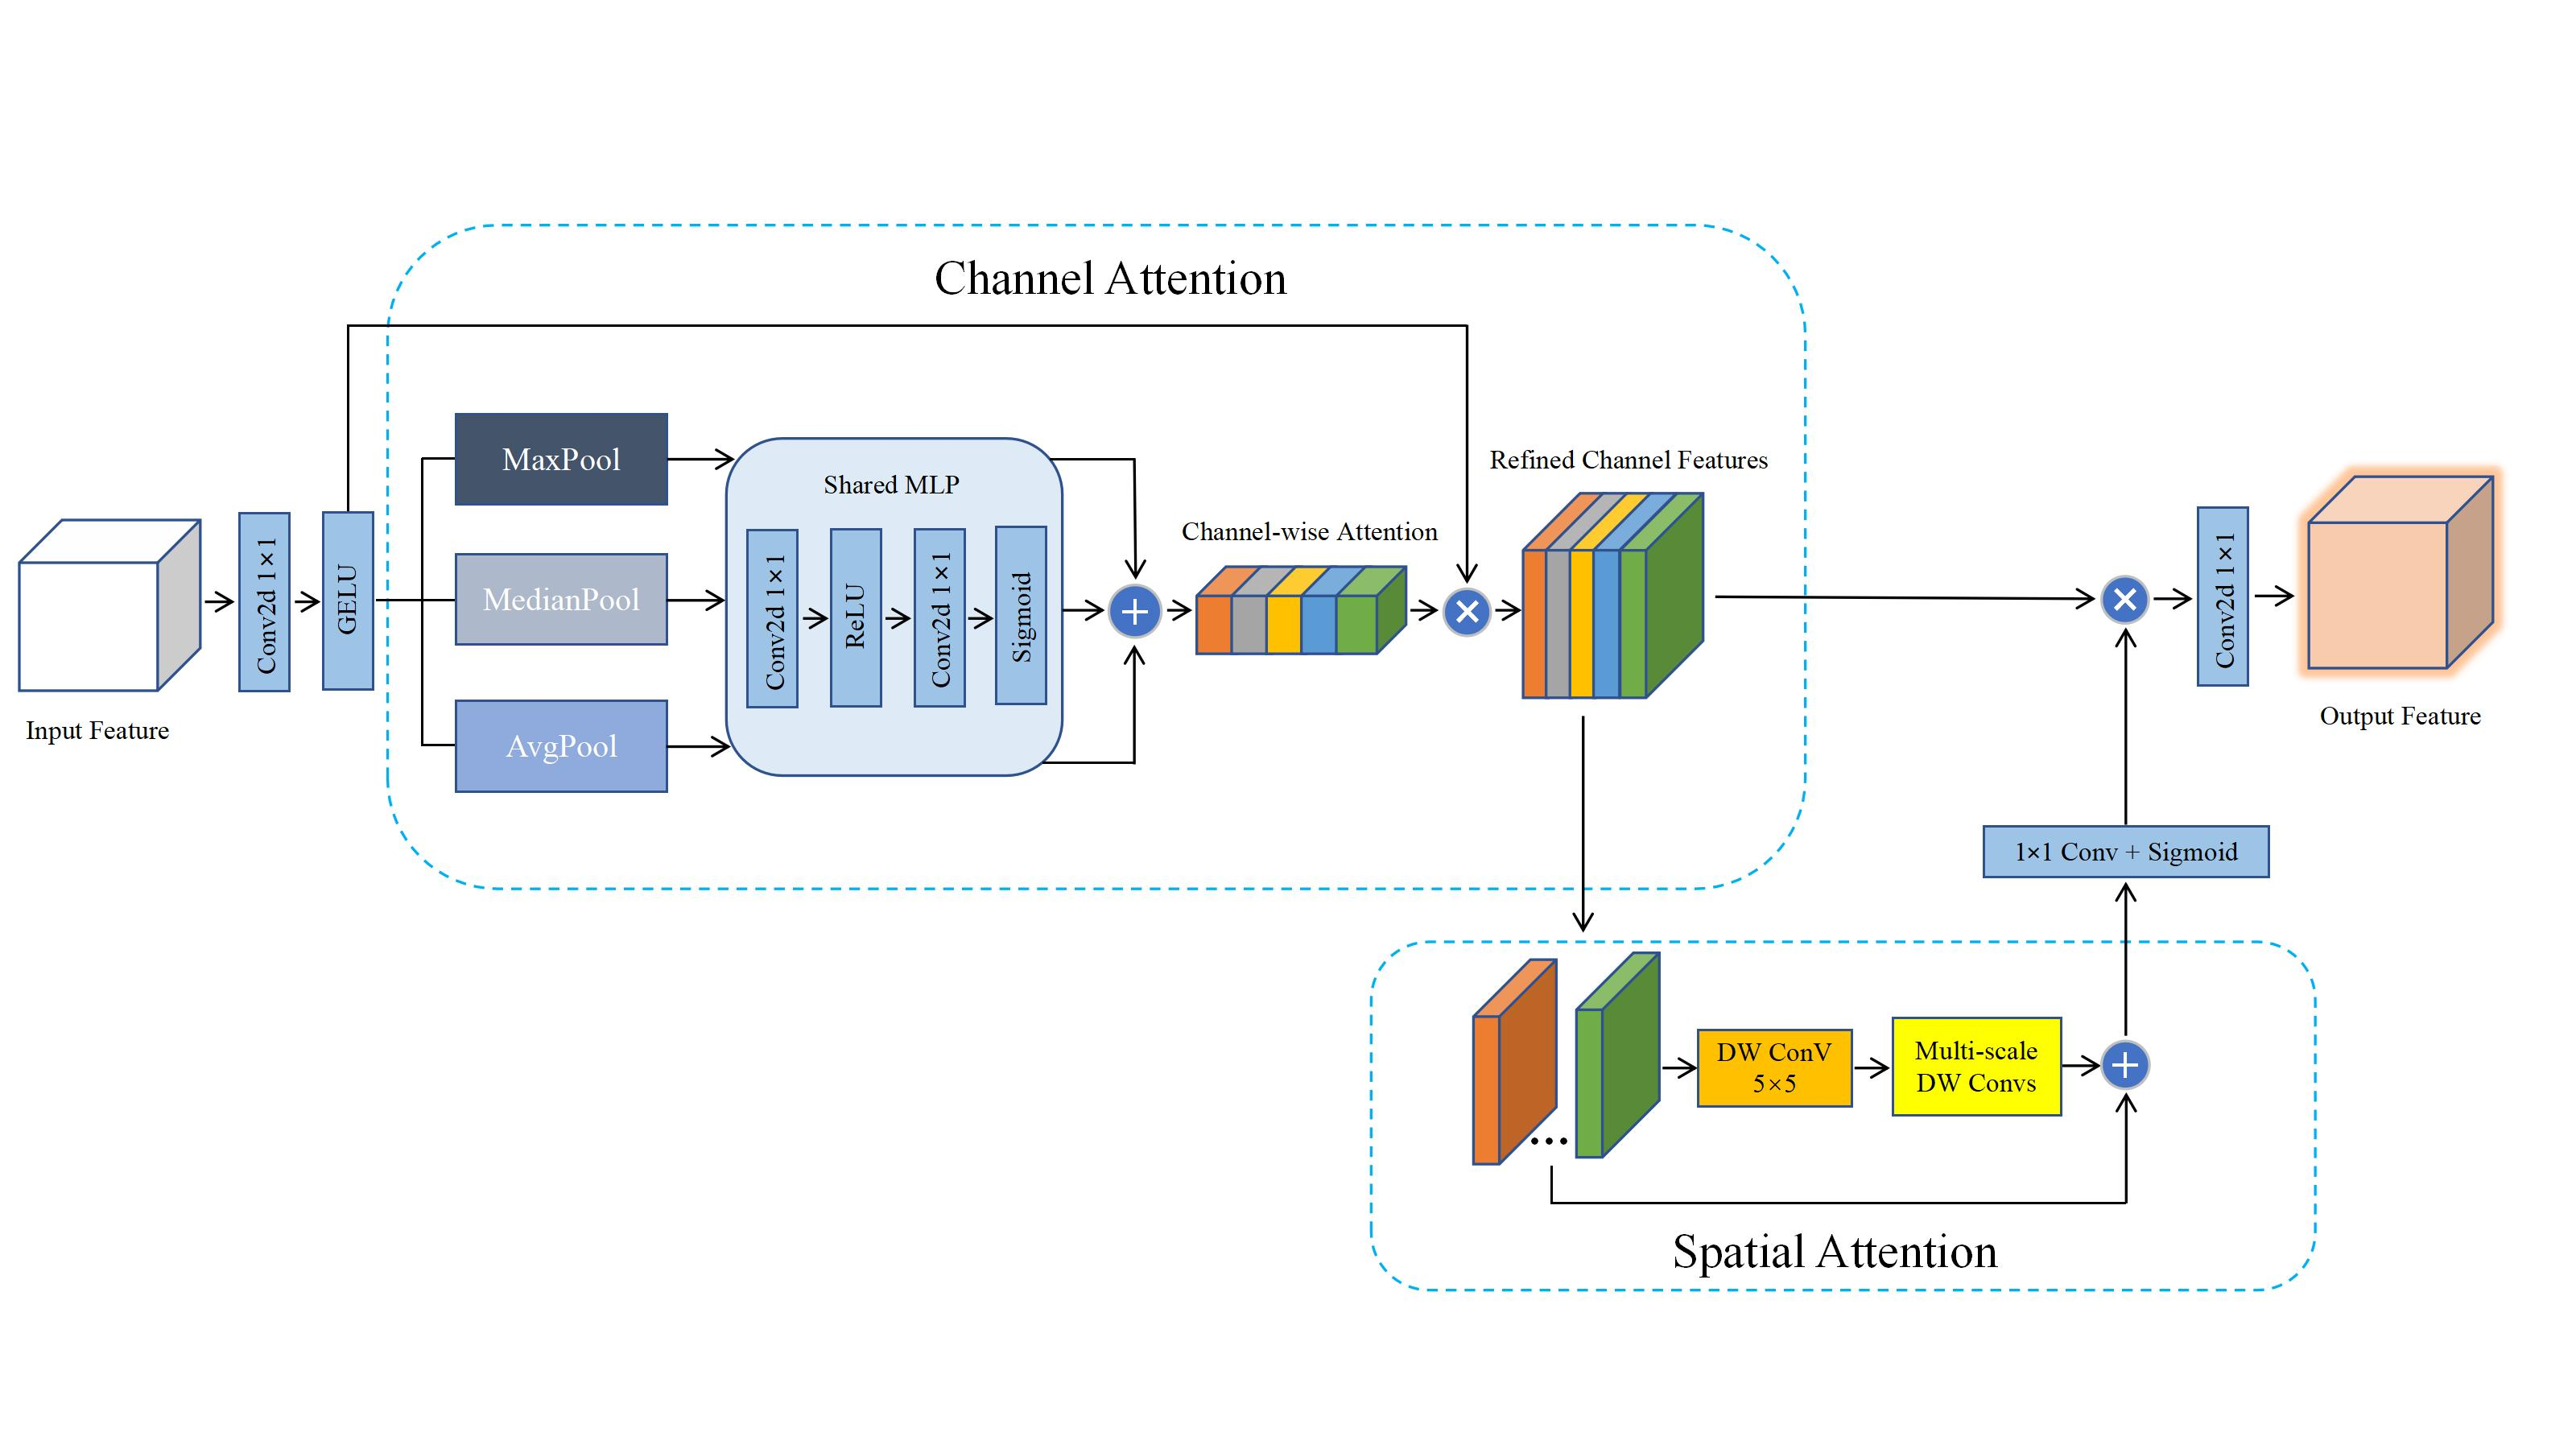
\includegraphics[width=0.92\linewidth]{fig_mesc_module.jpg}
    \caption{Illustration of the MESC module. The channel branch fuses global average, max, and median descriptors through a shared MLP. The spatial branch uses an initial \(5 \times 5\) depthwise convolution followed by six non-dilated directional depthwise branches with kernels \((1,7)\), \((7,1)\), \((1,11)\), \((11,1)\), \((1,21)\), and \((21,1)\). The symbols \(\oplus\) and \(\odot\) denote element-wise addition and broadcast multiplication, respectively.}
    \label{figurelabel1}
\end{figure}

\subsubsection{Spatial Attention: Multi-scale Modeling for Lesion Structure}

Lesions in medical images typically exhibit significant scale variations, and discriminative features often coexist at local and global levels. To capture such patterns with limited computational overhead, MESC uses depthwise convolutions. First, a \(5 \times 5\) depthwise convolution extracts local spatial context:

\begin{equation}
    U = D_{5\times5}(F_c).
\end{equation}
Then six non-dilated depthwise branches model horizontal and vertical context at three scales:

\begin{equation}
\begin{aligned}
    S = F_c \oplus
    D_{1\times7}(U) \oplus D_{7\times1}(U)
    \oplus D_{1\times11}(U) \oplus D_{11\times1}(U)
    \oplus D_{1\times21}(U) \oplus D_{21\times1}(U).
\end{aligned}
\end{equation}
The residual term \(F_c\) preserves the channel-refined feature while the depthwise branches aggregate multi-scale spatial evidence. The spatial attention map is estimated from \(S\), but the final attention reweights \(F_c\) rather than \(S\):
\begin{equation}
\begin{aligned}
    A_s &= \sigma\left(W_s^{1\times1}(S)\right),\\
    F_{\text{out}} &= W_o^{1\times1}\left(A_s \odot F_c\right).
\end{aligned}
\end{equation}
Thus, MESC adaptively enhances diagnostically relevant regions while retaining a lightweight module structure.

\subsection{Distance-Aware Soft Target Loss}

Medical grading tasks typically have a well-defined ordered structure, accompanied by non-negligible annotation uncertainty. Traditional cross-entropy loss treats each category as independent and fails to distinguish adjacent-grade errors from long-distance errors.

\begin{figure}[thpb]
    \centering
    % TODO: Regenerate Fig. 2 from the source diagram as vector PDF before camera-ready; only a raster source is available in this submission folder.
    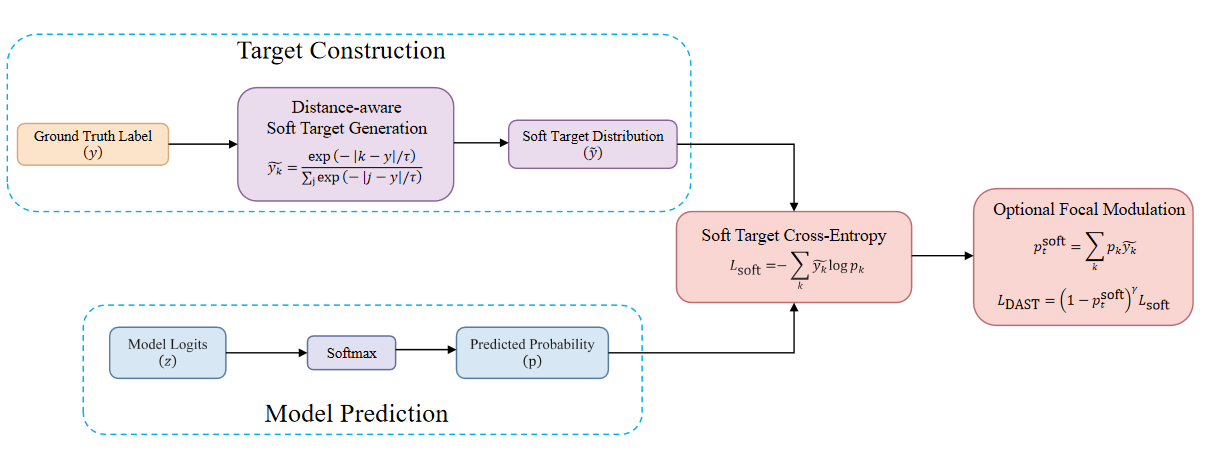
\includegraphics[width=0.92\linewidth]{fig_dast_loss.png}
    \caption{Illustration of DAST. For a ground-truth class \(y\), class distances \(d(k,y)=|k-y|\) are converted into a distance-decayed soft target distribution. The loss is applied to the original \(K\)-class softmax output and introduces no inference-time parameters.}
    \label{figurelabel2}
\end{figure}

Let \(y \in \{0,\ldots,K-1\}\) be the integer ground-truth class index and let \(p_k\) denote the predicted softmax probability of class \(k\). We define the class distance as
\begin{equation}
    d(k,y)=|k-y|.
\end{equation}
The DAST target distribution is constructed as

\begin{equation}
\begin{aligned}
    \tilde{y}_k =
    \frac{\exp\left(-d(k,y)/\tau\right)}
    {\sum_{j=0}^{K-1}\exp\left(-d(j,y)/\tau\right)}.
\end{aligned}
\end{equation}
Here, \(\tau>0\) controls the smoothness of the target distribution. A smaller \(\tau\) produces a sharper target concentrated around \(y\), whereas a larger \(\tau\) assigns more probability mass to neighboring classes.

The loss used in our experiments is a soft-target focal cross-entropy:

\begin{equation}
\begin{aligned}
    \mathcal{L}_{\text{DAST}}
    = - \left(1-\sum_{k=0}^{K-1}\tilde{y}_k p_k\right)^{\gamma}
    \sum_{k=0}^{K-1}\tilde{y}_k \log(p_k+\epsilon),
\end{aligned}
\end{equation}
where \(\gamma \ge 0\) is the focusing parameter and \(\epsilon\) is a small constant for numerical stability. The focal factor is applied at the sample level through \(1-\sum_k \tilde{y}_k p_k\), matching the implementation; it is not the class-wise form \(\sum_k \tilde{y}_k(1-p_k)^\gamma\log(p_k+\epsilon)\). When \(\gamma=0\), DAST reduces to soft-label cross-entropy with a distance-decayed target. A larger \(\gamma\) increases the contribution of samples whose probability mass is not aligned with the soft target.

DAST is mainly designed for ordinal grading tasks such as Knee Osteoarthritis KL grading, where adjacent labels have meaningful clinical proximity. On non-ordinal or weakly ordered datasets, the same objective should be interpreted more conservatively as a soft-target regularizer rather than a strict ordinal model.

\section{Experiments}
\subsection{Datasets and Evaluation Metrics}
\subsubsection{Datasets}
\begin{table}[H]
    \centering
    \caption{Broad comparison with representative classification backbones and the proposed ResNet50-based framework.}
    \label{tab:performance_comparison}
    \resizebox{\textwidth}{!}{
    \begin{tabular}{lcccccccccc}
    \toprule
    \multirow{3}{*}{Method} & \multicolumn{2}{c}{Bone Disease} & \multicolumn{2}{c}{Skin Disease} & \multicolumn{2}{c}{Lung Diseases} & \multicolumn{4}{c}{Brain Diseases} \\
    \cmidrule(lr){2-3} \cmidrule(lr){4-5} \cmidrule(lr){6-7} \cmidrule(lr){8-11}
    & \multicolumn{2}{c}{Knee Osteoarthritis} & \multicolumn{2}{c}{HAM10000} & \multicolumn{2}{c}{Chest X-ray Image} & \multicolumn{2}{c}{ADNI} & \multicolumn{2}{c}{Brain Tumor MRI} \\
    \cmidrule(lr){2-3} \cmidrule(lr){4-5} \cmidrule(lr){6-7} \cmidrule(lr){8-9} \cmidrule(lr){10-11}
    & ACC & F1-score & ACC & F1-score & ACC & F1-score & ACC & F1-score & ACC & F1-score \\
    \midrule
    VGG16 & 66.00 & 0.6600 & -- & -- & 92.22 & 0.9194 & 98.00 & 0.9801 & 90.97 & 0.8970 \\
    VGG19 & 64.00 & 0.5800 & -- & -- & 95.04 & 0.9504 & 97.11 & 0.9712 & 94.83 & 0.9470 \\
    Xception & -- & -- & -- & -- & 86.02 & 0.8526 & 82.66 & 0.8265 & 91.79 & 0.9018 \\
    Inception-ResNetV2 & 63.00 & 0.6000 & -- & -- & 86.51 & 0.8653 & 89.65 & 0.8739 & 90.66 & 0.9077 \\
    InceptionV3 & -- & -- & -- & -- & 86.82 & 0.8479 & 68.59 & 0.7017 & 88.15 & 0.8760 \\
    DenseNet121 & 64.00 & 0.5900 & -- & -- & 84.27 & 0.8020 & 89.53 & 0.8980 & 91.57 & 0.9041 \\
    DenseNet169 & -- & -- & -- & -- & 87.23 & 0.8652 & 95.94 & 0.9594 & 92.23 & 0.9223 \\
    DenseNet201 & -- & -- & -- & -- & 86.37 & 0.8731 & 92.34 & 0.9243 & 91.74 & 0.9174 \\
    MobileNetV2 & 67.00 & 0.6700 & -- & -- & 86.68 & 0.8576 & 68.28 & 0.6824 & 91.73 & 0.9160 \\
    ViT & -- & -- & -- & -- & 89.82 & 0.9000 & 93.70 & 0.9210 & 84.71 & 0.8500 \\
    ResNet101 & 69.00 & 0.6500 & -- & -- & 95.36 & 0.9538 & 96.48 & 0.9726 & 88.02 & 0.8620 \\
    ResNet50V2 & -- & -- & -- & -- & 89.02 & 0.8890 & 60.62 & 0.6034 & 90.77 & 0.9081 \\
    ResNet50 & 66.12 & 0.6659 & 88.32 & 0.8075 & 95.73 & 0.9562 & 94.45 & 0.9248 & 94.94 & 0.9482 \\
    ResNet layer3+MESC+DAST & 69.99 & 0.6956 & 89.27 & 0.8368 & 96.51 & 0.9680 & 98.91 & 0.9816 & 95.62 & 0.9554 \\
    \bottomrule
\end{tabular}
    }
    \vspace{0.2em}
    \begin{minipage}{0.98\textwidth}
    \footnotesize Table I is intended as a broad literature-style backbone comparison and should not be interpreted as a strictly controlled comparison of architectural modules, because the compared models differ in backbone design and parameter count. The controlled comparison is provided by the ResNet50-based ablation study in Table~\ref{tab:ablation_experiments}. The symbol ``--'' indicates that the value is unavailable in the current experimental record or was not reported under the same setting. Data sources: Knee Osteoarthritis~\cite{28}, HAM10000~\cite{40}, Chest X-ray Image~\cite{29,30}, ADNI-derived Alzheimer MRI~\cite{31,32,33,34}, Brain Tumor MRI~\cite{35,36,37,38,39}.
    \end{minipage}
\end{table}
We conduct experiments on five public medical image datasets covering skin lesion classification, chest X-ray disease recognition, Alzheimer MRI classification, brain tumor MRI classification, and knee osteoarthritis (KOA) severity grading. HAM10000 contains dermoscopic images from seven diagnostic categories: akiec, bcc, bkl, df, mel, nv, and vasc. We use a stratified split with 7210 training, 802 validation, and 2003 test images. Chest X-ray Image is a three-class radiograph dataset with COVID19, NORMAL, and PNEUMONIA classes. The raw training folder contains 5144 images, from which 4630/514 images are used for training/validation, and the independent test folder contains 1288 images. The ADNI-derived Alzheimer MRI benchmark contains four ordered disease-status classes: NonDemented, VeryMildDemented, MildDemented, and ModerateDemented. We use stratified splits with 4608 training, 512 validation, and 1280 test images.

Brain Tumor MRI is treated as the MRI dataset used in this work. It contains four classes, glioma, meningioma, notumor, and pituitary. The original training folder contains 5600 images with 1400 images per class, and 10\% of this folder is stratified into validation, producing 5040 training and 560 validation images. The test folder contains 1600 images, with 400 images per class. The Knee Osteoarthritis dataset is an ordinal grading task annotated by KL grades 0--4, corresponding to normal, doubtful, mild, moderate, and severe cases. We use the provided split with 5778 training, 826 validation, and 1656 test images.

\begin{table}[H]
    \centering
    \caption{Dataset statistics and evaluation protocol.}
    \label{tab:dataset_statistics}
    \scriptsize
    \setlength{\tabcolsep}{3pt}
    \begin{tabular}{p{0.16\textwidth}p{0.42\textwidth}p{0.25\textwidth}p{0.12\textwidth}}
        \toprule
        Dataset & Modality, classes, and train/val/test split & Preprocessing & Metrics \\
        \midrule
        HAM10000 & Dermoscopy; 7 classes: akiec, bcc, bkl, df, mel, nv, vasc; 7210/802/2003 & Resize 224; ImageNet normalization; flip/rotation & ACC, macro-F1 \\
        Chest X-ray Image & X-ray; 3 classes: COVID19, NORMAL, PNEUMONIA; 4630/514/1288 & Grayscale-to-RGB; resize 224; ImageNet normalization; flip/rotation & ACC, macro-F1 \\
        ADNI-derived Alzheimer MRI & MRI; 4 classes: NonDemented, VeryMildDemented, MildDemented, ModerateDemented; 4608/512/1280 & Grayscale-to-RGB; resize 224; ImageNet normalization; flip/rotation & ACC, macro-F1, QWK, MAE \\
        Brain Tumor MRI & MRI; 4 classes: glioma, meningioma, notumor, pituitary; 5040/560/1600 & Resize 224; ImageNet normalization; flip/rotation/color jitter & ACC, macro-F1 \\
        Knee Osteoarthritis & X-ray; 5 KL grades: normal, doubtful, mild, moderate, severe; 5778/826/1656 & Grayscale-to-RGB; resize 224; ImageNet normalization; flip/rotation & ACC, macro-F1, QWK, MAE, 1-off ACC \\
        \bottomrule
    \end{tabular}
\end{table}

For all datasets, images are resized to \(224 \times 224\). RGB datasets are normalized with ImageNet mean and standard deviation. Grayscale medical images are converted to three channels before normalization. Training augmentation includes random horizontal flipping and mild rotation; Brain Tumor MRI additionally uses light color jitter. Evaluation uses deterministic resizing and normalization. Accuracy and macro F1-score are used as the main metrics, with QWK and MAE additionally monitored for ordinal datasets.


\subsubsection{Evaluation Metrics}

We evaluate model performance using two standard metrics: Accuracy and F1-score. Accuracy measures the overall classification correctness, while F1-score provides a more balanced assessment by jointly considering precision and recall, making it more suitable for medical imaging tasks with class imbalance. This combination ensures both global performance evaluation and sensitivity to minority classes across all datasets.

\subsection{Comparative Evaluation with Baselines}
\subsubsection{Experimental Setup}
To evaluate the effectiveness of the proposed method, we compare it with a ResNet50 baseline and representative classification backbones. Table~\ref{tab:performance_comparison} is used as a broad backbone-level comparison and is not a strictly controlled module comparison. The controlled experiments use the same ResNet50 backbone and are reported in Table~\ref{tab:ablation_experiments}. In the controlled setting, MESC is inserted after \textit{layer3}. Models are trained with Adam or AdamW according to the dataset runner, input images are resized to \(224 \times 224\), and early stopping is applied using validation performance. Unless otherwise stated, experiments use seed 1234, train for up to 50--60 epochs, use a batch size of 16 or 32 depending on GPU memory and dataset runner, and retain the best validation checkpoint for test evaluation. DAST uses \(\tau=1.0\) and \(\gamma=1.5\) by default; the tuned Brain Tumor MRI run uses \(\tau=1.5\) and \(\gamma=2.0\), selected on validation performance.

Repeated-seed logs are not available for all datasets in the current experimental record. Therefore, Tables~\ref{tab:performance_comparison} and~\ref{tab:ablation_experiments} report single-run test results selected by validation performance. For future statistical validation, each controlled setting should be repeated over at least three independent seeds and reported as mean \(\pm\) standard deviation, with paired significance tests such as a paired \(t\)-test or Wilcoxon signed-rank test applied to matched-seed results. Hyperparameter sensitivity is kept to a single seed to reduce training cost and is used only for validation-set selection.

\begin{table}[H]
    \centering
    \caption{Model complexity measured with batch size 1 and \(224 \times 224\) input. FLOPs are counted for convolution and linear layers, and inference time is measured on CPU using the provided complexity script.}
    \label{tab:model_complexity}
    \scriptsize
    \begin{tabular}{lcccc}
        \toprule
        Method & Parameters & FLOPs & Inference time & Input size \\
        \midrule
        ResNet50 & 23.52M & 4.09G & 26.57 ms & \(224 \times 224\) \\
        ResNet50 + MESC (layer3) & 27.31M & 4.73G & 32.49 ms & \(224 \times 224\) \\
        ResNet50 + MESC (layer3) + DAST & 27.31M & 4.73G & 33.30 ms & \(224 \times 224\) \\
        \bottomrule
    \end{tabular}
\end{table}


\subsubsection{Result Analysis}
As shown in Table~\ref{tab:performance_comparison}, the proposed ResNet50-based framework achieves competitive performance among the evaluated baselines. Compared with the ResNet50 baseline under the same experimental setting, it improves performance on Knee Osteoarthritis, HAM10000, Chest X-ray Image, ADNI-derived Alzheimer MRI, and Brain Tumor MRI. This trend is consistent with the design motivation of MESC, which enhances feature representation through robust channel recalibration and multi-scale spatial modeling. On Knee Osteoarthritis, the improvement is also supported by the ordinal nature of KL grading, where the distance-aware supervision of DAST can reduce severe long-distance mistakes.

\subsection{Ablation Study}
\subsubsection{Experimental Setup}

To further verify the effectiveness of each component in the proposed method, ablation experiments were conducted on five medical imaging datasets, namely Knee Osteoarthritis, HAM10000, Chest X-ray Image, ADNI, and Brain Tumor MRI, under the following four settings:
 
 \begin{enumerate}
    \item ResNet Baseline;
    \item ResNet Baseline + DAST;
    \item ResNet layer3 + MESC;
    \item ResNet layer3 + MESC + DAST.
\end{enumerate}
 
 Among them, Baseline + DAST is used to verify the role of distance-aware soft label loss in different tasks, layer3 + MESC is used to verify the enhancement effect of the mid-high level feature enhancement module on the representation ability of medical images, while the complete model is used to analyze the complementarity when the structural module and loss function are used in combination. Through this disassembly approach, it is possible to more clearly illustrate the contributions brought by the two core improvements proposed in this paper, namely MESC and DAST, respectively, and whether their combination can further improve the model performance.


\subsubsection{Result Analysis}

\begin{table}[H]
    \centering
    \caption{Controlled ResNet50-based ablation experiments of MESC and DAST.}
    \label{tab:ablation_experiments}
    \resizebox{\textwidth}{!}{
    \begin{tabular}{lcccccccccc}
        \toprule
        \multirow{3}{*}{Method} & \multicolumn{2}{c}{Bone Disease} & \multicolumn{2}{c}{Skin Disease} & \multicolumn{2}{c}{Lung Diseases} & \multicolumn{4}{c}{Brain Diseases} \\
        \cmidrule(lr){2-3} \cmidrule(lr){4-5} \cmidrule(lr){6-7} \cmidrule(lr){8-11}
        & \multicolumn{2}{c}{Knee Osteoarthritis} & \multicolumn{2}{c}{HAM10000} & \multicolumn{2}{c}{Chest X-ray Image} & \multicolumn{2}{c}{ADNI} & \multicolumn{2}{c}{Brain Tumor MRI} \\
        \cmidrule(lr){2-3} \cmidrule(lr){4-5} \cmidrule(lr){6-7} \cmidrule(lr){8-9} \cmidrule(lr){10-11}
        & ACC & F1-score & ACC & F1-score & ACC & F1-score & ACC & F1-score & ACC & F1-score \\
        \midrule
        ResNet Baseline & 66.12 & 0.6659 & 88.32 & 0.8075 & 95.73 & 0.9562 & 94.45 & 0.9248 & 94.94 & 0.9482 \\
        ResNet Baseline + DAST & 67.03 & 0.6691 & 89.07 & 0.8288 & 96.12 & 0.9630 & 93.28 & 0.9283 & 95.19 & 0.9506 \\
        ResNet layer3 + MESC & 68.84 & 0.6762 & 89.62 & 0.8337 & 96.51 & 0.9679 & 98.59 & 0.9787 & 95.19 & 0.9507 \\
        \textbf{ResNet layer3 + MESC + DAST} & \textbf{69.99} & \textbf{0.6956} & \textbf{89.27} & \textbf{0.8368} & \textbf{96.51} & \textbf{0.9680} & \textbf{98.91} & \textbf{0.9816} & \textbf{95.62} & \textbf{0.9554} \\
        \bottomrule
    \end{tabular}
    }
\end{table}
As shown in Table~\ref{tab:ablation_experiments}, MESC provides the most stable gains across the evaluated datasets. Adding MESC to ResNet50 improves or maintains both ACC and macro F1 on Knee Osteoarthritis, HAM10000, Chest X-ray Image, ADNI-derived Alzheimer MRI, and Brain Tumor MRI. This supports the hypothesis that robust channel statistics and multi-scale spatial modeling improve mid-to-high level medical image representations.

DAST has a more task-dependent effect. It is most meaningful for ordered label spaces, especially Knee Osteoarthritis, where neighboring KL grades have clinical proximity and long-distance errors are more severe. On non-ordinal or weakly ordered datasets, DAST behaves mainly as a soft-target regularizer and can interact with class semantics or imbalance. For example, HAM10000 shows an accuracy/F1 trade-off: MESC alone gives higher accuracy, whereas MESC+DAST gives slightly higher macro F1. ADNI-derived Alzheimer MRI also indicates that DAST alone is not universally beneficial, because ResNet Baseline + DAST reduces ACC compared with the ResNet50 baseline. Therefore, MESC+DAST should be interpreted as generally effective in the evaluated settings rather than universally complementary for every dataset.

DAST has a small number of hyperparameters, so the accompanying experiment scripts include a single-seed Knee Osteoarthritis sensitivity grid for \(\tau \in \{0.5,1.0,1.5,2.0\}\) and \(\gamma \in \{0.0,1.0,1.5,2.0\}\). This grid is intended for validation-set model selection rather than statistical significance testing.

\subsection{Grad-CAM Analysis}

To further investigate the interpretability of the proposed model, we visualize representative samples from five datasets using Grad-CAM, as shown in Fig.~\ref{fig:gradcam}. In these examples, high-response regions are generally aligned with clinically meaningful image regions rather than only background areas. For instance, in skin lesion images, high-response regions concentrate on lesion areas and boundaries; in chest X-ray images, activations align with abnormal pulmonary regions; in ADNI-derived Alzheimer MRI images, the model attends to brain regions related to disease-associated structural patterns; and in Brain Tumor MRI, responses are localized around tumor-related regions. These observations provide qualitative evidence that the proposed method can capture meaningful visual patterns across diverse imaging modalities.

For the knee osteoarthritis grading task, the activation patterns further reflect sensitivity to structural variations. The model primarily attends to key anatomical regions such as joint spaces and adjacent bone structures, and its focus shifts with disease severity, from subtle localized responses in early stages to more concentrated patterns in advanced cases. This suggests that the model not only learns discriminative features but also captures progression-related cues, providing interpretable support for its predictions.


\begin{figure}[htbp]
    \centering

    \begin{subfigure}[b]{0.32\linewidth}
        \centering
        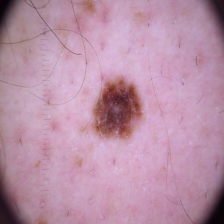
\includegraphics[width=\linewidth]{ham10000_a.png}
        \vspace{0.2em}
        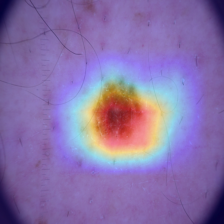
\includegraphics[width=\linewidth]{ham10000_b.png}
        \caption{HAM10000}
    \end{subfigure}
    \hfill
    \begin{subfigure}[b]{0.32\linewidth}
        \centering
        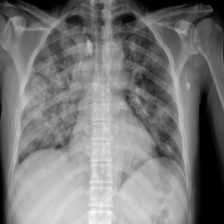
\includegraphics[width=\linewidth]{chest_xray_a.png}
        \vspace{0.2em}
        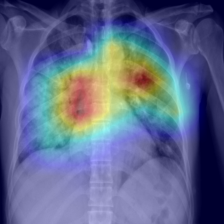
\includegraphics[width=\linewidth]{chest_xray_b.png}
        \caption{Chest X-ray}
    \end{subfigure}
    \hfill
    \begin{subfigure}[b]{0.32\linewidth}
        \centering
        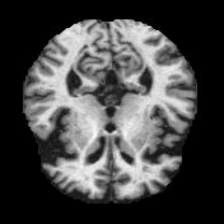
\includegraphics[width=\linewidth]{adni_a.png}
        \vspace{0.2em}
        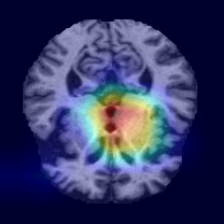
\includegraphics[width=\linewidth]{adni_b.png}
        \caption{ADNI}
    \end{subfigure}

    \vspace{0.8em}

    \begin{subfigure}[b]{0.32\linewidth}
        \centering
        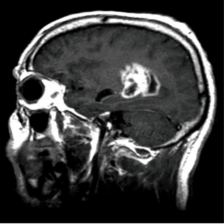
\includegraphics[width=\linewidth]{brain_tumor_a.png}
        \vspace{0.2em}
        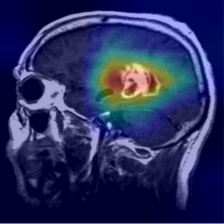
\includegraphics[width=\linewidth]{brain_tumor_b.png}
        \caption{Brain Tumor MRI}
    \end{subfigure}
    \hfill
    \begin{subfigure}[b]{0.32\linewidth}
        \centering
        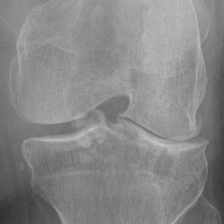
\includegraphics[width=\linewidth]{knee_osteo_1.png}
        \vspace{0.2em}
        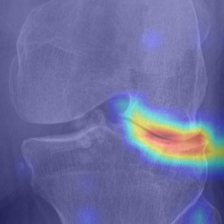
\includegraphics[width=\linewidth]{knee_osteo_2.png}
        \caption{Knee (Moderate)}
    \end{subfigure}
    \hfill
        \begin{subfigure}[b]{0.32\linewidth}
        \centering
        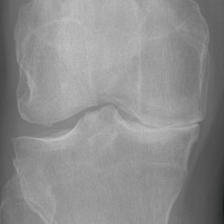
\includegraphics[width=\linewidth]{knee_osteo_3.png}
        \vspace{0.2em}
        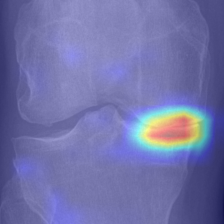
\includegraphics[width=\linewidth]{knee_osteo_4.png}
        \caption{Knee (Severe)}
    \end{subfigure}
    
    \caption{Grad-CAM visualization on five representative datasets. For each pair, the original image is shown above the corresponding activation map. The examples illustrate that the model often attends to lesion, organ, tumor, or joint regions that are relevant to the target task.}
    \label{fig:gradcam}
\end{figure}


   

\section{Conclusion}

This paper proposes a unified framework for medical image classification and grading to address the limitations of existing methods in complex structural representation and inter-class relationship modeling. Specifically, we introduce a Median-enhanced Spatial and Channel Attention (MESC) module, which improves the representation of key lesion regions and structural patterns by integrating multiple statistical cues with multi-scale spatial modeling. In addition, we propose a Distance-Aware Soft Target (DAST) loss, which explicitly incorporates inter-class distance information into training, enabling the model to distinguish adjacent errors from long-distance misclassifications in a more reasonable manner.
Experimental results on HAM10000, Chest X-ray Image, ADNI-derived Alzheimer MRI, Brain Tumor MRI, and Knee Osteoarthritis show that the proposed framework improves over the ResNet50 baseline under the same experimental setting and achieves competitive performance among the evaluated baselines. The ablation study further indicates that MESC provides stable gains across datasets, whereas DAST is most beneficial for ordered label spaces such as Knee Osteoarthritis. On non-ordinal datasets, DAST should be interpreted as a soft-target regularizer whose effect can depend on class semantics and imbalance.
Overall, the results suggest that feature enhancement and structured supervision can address complementary aspects of medical image classification and grading, but their interaction is not universally positive for every dataset. Future work will focus on lighter module design, stronger cross-dataset generalization, complete multi-seed statistical validation, and clinically realistic external evaluation.







\begin{thebibliography}{99}
\bibitem{1} B. Sistaninejhad, H. Rasi, and P. Nayeri, “A Review Paper about Deep Learning for Medical Image Analysis,” Computational and Mathematical Methods in Medicine, vol. 2023, no. 1, Jan. 2023, doi: 10.1155/2023/7091301.

\bibitem{2} M. D. Kohn, A. A. Sassoon, and N. D. Fernando, “Classifications in Brief: Kellgren-Lawrence Classification of Osteoarthritis,” Clinical Orthopaedics \& Related Research, vol. 474, no. 8, pp. 1886–1893, Aug. 2016, doi: 10.1007/s11999-016-4732-4.

\bibitem{3} P. Chen, L. Gao, X. Shi, K. Allen, and L. Yang, “Fully automatic knee osteoarthritis severity grading using deep neural networks with a novel ordinal loss,” Computerized Medical Imaging and Graphics, vol. 75, pp. 84–92, Jul. 2019, doi: 10.1016/j.compmedimag.2019.06.002.

\bibitem{4} K. He, X. Zhang, S. Ren, and J. Sun, “Deep Residual Learning for Image Recognition,” 2016 IEEE Conference on Computer Vision and Pattern Recognition (CVPR), pp. 770–778, Jun. 2016, doi: 10.1109/cvpr.2016.90.

\bibitem{5} J. Hu, L. Shen, and G. Sun, “Squeeze-and-Excitation Networks,” 2018 IEEE/CVF Conference on Computer Vision and Pattern Recognition, pp. 7132–7141, Jun. 2018, doi: 10.1109/cvpr.2018.00745.

\bibitem{6} S. Woo, J. Park, J.-Y. Lee, and I. S. Kweon, “CBAM: Convolutional Block Attention Module,” Computer Vision – ECCV 2018, pp. 3–19, 2018, doi: 10.1007/978-3-030-01234-2\_1.

\bibitem{7} B. Zhang, J. Tan, K. Cho, G. Chang, and C. M. Deniz, “Attention-based CNN for KL Grade Classification: Data from the Osteoarthritis Initiative,” 2020 IEEE 17th International Symposium on Biomedical Imaging (ISBI), pp. 731–735, Apr. 2020, doi: 10.1109/isbi45749.2020.9098456.

\bibitem{8} R. K. Jain, P. K. Sharma, S. Gaj, A. Sur, and P. Ghosh, “Knee osteoarthritis severity prediction using an attentive multi-scale deep convolutional neural network,” Multimedia Tools and Applications, vol. 83, no. 3, pp. 6925–6942, Jun. 2023, doi: 10.1007/s11042-023-15484-w.

\bibitem{9} R. Díaz and A. Marathe, “Soft Labels for Ordinal Regression,” 2019 IEEE/CVF Conference on Computer Vision and Pattern Recognition (CVPR), pp. 4733–4742, Jun. 2019, doi: 10.1109/cvpr.2019.00487.

\bibitem{10} W. Tang, Z. Yang, and Y. Song, “Disease-grading networks with ordinal regularization for medical imaging,” Neurocomputing, vol. 545, p. 126245, Aug. 2023, doi: 10.1016/j.neucom.2023.126245.

\bibitem{11} R. Müller, S. Kornblith, and G. Hinton, “When does label smoothing help?,” arXiv preprint arXiv:1906.02629, 2019.

\bibitem{12} J. Antony, K. McGuinness, N. E. O’Connor, and K. Moran, “Quantifying radiographic knee osteoarthritis severity using deep convolutional neural networks,” 2016 23rd International Conference on Pattern Recognition (ICPR), pp. 1195–1200, Dec. 2016, doi: 10.1109/icpr.2016.7899799.

\bibitem{13} C. Szegedy et al., “Going deeper with convolutions,” 2015 IEEE Conference on Computer Vision and Pattern Recognition (CVPR), pp. 1–9, Jun. 2015, doi: 10.1109/cvpr.2015.7298594.

\bibitem{14} F. Chollet, “Xception: Deep Learning with Depthwise Separable Convolutions,” 2017 IEEE Conference on Computer Vision and Pattern Recognition (CVPR), pp. 1800–1807, Jul. 2017, doi: 10.1109/cvpr.2017.195.

\bibitem{15} M. Sandler, A. Howard, M. Zhu, A. Zhmoginov, and L.-C. Chen, “MobileNetV2: Inverted Residuals and Linear Bottlenecks,” 2018 IEEE/CVF Conference on Computer Vision and Pattern Recognition, pp. 4510–4520, Jun. 2018, doi: 10.1109/cvpr.2018.00474.

\bibitem{16} X. Wang, R. Girshick, A. Gupta, and K. He, “Non-local Neural Networks,” 2018 IEEE/CVF Conference on Computer Vision and Pattern Recognition, pp. 7794–7803, Jun. 2018, doi: 10.1109/cvpr.2018.00813.

\bibitem{17} T.-Y. Lin, P. Goyal, R. Girshick, K. He, and P. Dollar, “Focal Loss for Dense Object Detection,” 2017 IEEE International Conference on Computer Vision (ICCV), pp. 2999–3007, Oct. 2017, doi: 10.1109/iccv.2017.324.

\bibitem{18} A. Tiulpin, J. Thevenot, E. Rahtu, P. Lehenkari, and S. Saarakkala, “Automatic Knee Osteoarthritis Diagnosis from Plain Radiographs: A Deep Learning-Based Approach,” Scientific Reports, vol. 8, no. 1, Jan. 2018, doi: 10.1038/s41598-018-20132-7.

\bibitem{19} A. Tiulpin and S. Saarakkala, “Automatic Grading of Individual Knee Osteoarthritis Features in Plain Radiographs Using Deep Convolutional Neural Networks,” Diagnostics, vol. 10, no. 11, p. 932, Nov. 2020, doi: 10.3390/diagnostics10110932.

\bibitem{20} S.-W. Pi, B.-D. Lee, M. S. Lee, and H. J. Lee, “Ensemble deep-learning networks for automated osteoarthritis grading in knee X-ray images,” Scientific Reports, vol. 13, no. 1, Dec. 2023, doi: 10.1038/s41598-023-50210-4.

\bibitem{21} H. Gu, K. Li, R. J. Colglazier, J. Yang, M. Lebhar, J. O’Donnell, W. A. Jiranek, R. C. Mather, R. J. French, N. Said, J. Zhang, C. Park, and M. A. Mazurowski, “Knee arthritis severity measurement using deep learning: A publicly available algorithm with a multi-institutional validation showing radiologist-level performance,” arXiv preprint arXiv:2203.08914, Mar. 2022.

\bibitem{22} Z. Wang et al., “Confidence-Driven Deep Learning Framework for Early Detection of Knee Osteoarthritis,” IEEE Transactions on Biomedical Engineering, vol. 73, no. 2, pp. 530–541, Feb. 2026, doi: 10.1109/tbme.2025.3587003.

\bibitem{23} A. Kurz et al., “Uncertainty Estimation in Medical Image Classification: Systematic Review,” JMIR Medical Informatics, vol. 10, no. 8, p. e36427, Aug. 2022, doi: 10.2196/36427.

\bibitem{24} A. Jungo et al., “On the Effect of Inter-observer Variability for a Reliable Estimation of Uncertainty of Medical Image Segmentation,” Medical Image Computing and Computer Assisted Intervention – MICCAI 2018, pp. 682–690, 2018, doi: 10.1007/978-3-030-00928-1\_77.

\bibitem{25} J. Lourenço-Silva and A. L. Oliveira, “Using Soft Labels to Model Uncertainty in Medical Image Segmentation,” Brainlesion: Glioma, Multiple Sclerosis, Stroke and Traumatic Brain Injuries, pp. 585–596, 2022, doi: 10.1007/978-3-031-09002-8\_52.

\bibitem{26} J. Zhang, Y. Zheng, and Y. Shi, “A Soft Label Method for Medical Image Segmentation with Multirater Annotations,” Computational Intelligence and Neuroscience, vol. 2023, no. 1, Jan. 2023, doi: 10.1155/2023/1883597.

\bibitem{27} F. C. Ghesu et al., “Quantifying and leveraging predictive uncertainty for medical image assessment,” Medical Image Analysis, vol. 68, p. 101855, Feb. 2021, doi: 10.1016/j.media.2020.101855.

\bibitem{28} A. S. Mohammed, A. A. Hasanaath, G. Latif, and A. Bashar, “Knee Osteoarthritis Detection and Severity Classification Using Residual Neural Networks on Preprocessed X-ray Images,” \textit{Diagnostics}, vol. 13, no. 8, p. 1380, 2023, doi: 10.3390/diagnostics13081380.

\bibitem{29} M. E. H. Chowdhury et al., “Can AI Help in Screening Viral and COVID-19 Pneumonia?,” IEEE Access, vol. 8, pp. 132665–132676, 2020, doi: 10.1109/access.2020.3010287.

\bibitem{30} G. I. Okolo, S. Katsigiannis, T. Althobaiti, and N. Ramzan, “On the Use of Deep Learning for Imaging-Based COVID-19 Detection Using Chest X-rays,” Sensors, vol. 21, no. 17, p. 5702, Aug. 2021, doi: 10.3390/s21175702.

\bibitem{31} R. Agarwal, A. S. Sathwik, D. Godavarthi, and J. V. Naga Ramesh, “Comparative Analysis of Deep Learning Models for Multiclass Alzheimer’s Disease Classification,” EAI Endorsed Transactions on Pervasive Health and Technology, vol. 9, Nov. 2023, doi: 10.4108/eetpht.9.4334.

\bibitem{32} A. Loddo, S. Buttau, and C. Di Ruberto, “Deep learning based pipelines for Alzheimer’s disease diagnosis: A comparative study and a novel deep-ensemble method,” Computers in Biology and Medicine, vol. 141, p. 105032, Feb. 2022, doi: 10.1016/j.compbiomed.2021.105032.

\bibitem{33} Y. Lyu, X. Yu, D. Zhu, and L. Zhang, “Classification of Alzheimer’s Disease via Vision Transformer,” Proceedings of the 15th International Conference on PErvasive Technologies Related to Assistive Environments, pp. 463–468, Jun. 2022, doi: 10.1145/3529190.3534754.

\bibitem{34} G. Sharma, A. Vijayvargiya, and R. Kumar, “Comparative Assessment among Different Convolutional Neural Network Architectures for Alzheimer’s Disease Detection,” 2021 IEEE 8th Uttar Pradesh Section International Conference on Electrical, Electronics and Computer Engineering (UPCON), pp. 1–6, Nov. 2021, doi: 10.1109/upcon52273.2021.9667607.

\bibitem{35} Balaji, R. Sen, and H. Kirty, “Detection and Classification of Brain Tumors Using Deep Convolutional Neural Networks,” arXiv preprint arXiv:2208.13264, 2022.

\bibitem{36} Md. A. A. Khandaker, Z. S. Raha, S. B. Iqbal, M. F. Mridha, and J. Shin, “From Images to Insights: Transforming Brain Cancer Diagnosis with Explainable AI,” 2024 27th International Conference on Computer and Information Technology (ICCIT), pp. 891–896, Dec. 2024, doi: 10.1109/iccit64611.2024.11022512.

\bibitem{37} H. Mehnatkesh, S. M. J. Jalali, A. Khosravi, and S. Nahavandi, “An intelligent driven deep residual learning framework for brain tumor classification using MRI images,” Expert Systems with Applications, vol. 213, p. 119087, Mar. 2023, doi: 10.1016/j.eswa.2022.119087.

\bibitem{38} Z. Rasheed et al., “Brain Tumor Classification from MRI Using Image Enhancement and Convolutional Neural Network Techniques,” Brain Sciences, vol. 13, no. 9, p. 1320, Sep. 2023, doi: 10.3390/brainsci13091320.

\bibitem{39} M. A. Talukder, M. M. Islam, and M. A. Uddin, “An Optimized Ensemble Deep Learning Model for Brain Tumor Classification,” arXiv preprint arXiv:2305.12844, 2024.

\bibitem{40} P. Tschandl, C. Rosendahl, and H. Kittler, "The HAM10000 dataset, a large collection of multi-source dermatoscopic images of common pigmented skin lesions," Scientific Data, vol. 5, Article 180161, 2018.

\end{thebibliography}

\end{document}
